\documentclass[12pt]{article}

\usepackage[utf8]{inputenc}
\usepackage{color}
\usepackage[T1]{fontenc}
\usepackage[french]{babel}
\usepackage{listings}
\usepackage{graphicx}
\usepackage[export]{adjustbox}
\usepackage{hyperref}
\usepackage{url}
\usepackage[nottoc,numbib]{tocbibind}
\usepackage{pgfgantt}
\usepackage{float}

\usetikzlibrary{babel}

\graphicspath{{figures/}}

\bibliographystyle{alpha}

\renewcommand{\listoffigures}{\begingroup
\tocsection
\tocfile{\listfigurename}{lof}
\endgroup}



\title {Solveurs et générateurs pour
	\\ des jeux de logique
	\\ \large Analyse des besoins}
    
\author{Martial DUVERNEIX, Florian GAUTIER, Pierre LORSON, Teiki PEPIN}


\begin{document}

\maketitle
\newpage

\tableofcontents
\newpage

\section{Introduction}

\subsection{Présentation du projet}

Ce projet consiste à concevoir des programmes pouvant générer et résoudre des instances des jeux de logique \textit{Hashiwokakero} et \textit{Inshi no heya}. De manière similaire au \textit{Sudoku}, ces deux jeux proviennent du journal japonais Nikoli et sont structurés sous forme d'une grille qui se complète à l'aide d'un crayon.\\

Dans le cadre de ce projet, on souhaite généraliser les méthodes implémentées pour la résolution et la génération de telle façon que la grille de jeu puisse avoir des dimensions variables. 

De plus, la résolution de ces puzzles devra être optimisée. Il sera nécessaire d'utiliser des méthodes proches de celles des solveurs SAT : il faut déterminer une valuation de variables booléennes exprimants les contraintes de la grille de jeu telle que toutes les contraintes soient satisfaites.\\

\subsection{Description des jeux de logiques}

\textit{Hashiwokakero} \cite{NikHashi18} est composé d'îles contenant des chiffres allant de 1 à 8. Il faut relier toutes les îles par des "ponts" pour former un seul groupe (figure \ref{fig:hashiwokakero}). Les ponts doivent être en ligne droite, ne peuvent pas se croiser entre eux et ne peuvent pas survoler une île. Chaque île doit avoir exactement autant de ponts que le nombre qu'elle indique. Dans la variante originale du jeu, deux îles ne peuvent pas être connectées directement entre elles par plus de deux ponts.

\begin{figure}[H]
\caption{Étapes de résolution du puzzle \textit{Hashiwokakero}.}
\label{fig:hashiwokakero}
\centering
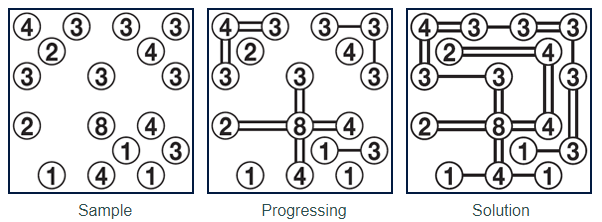
\includegraphics[width=.85\textwidth]{hashiwokakero}
\end{figure}

\textit{Inshi no heya} \cite{NikInshi18} contient des "salles" délimitées par des traits épais avec un nombre écrit en haut à gauche. Ces salles ont l'une de leurs dimensions (la largeur ou la longueur de la salle) fixée à une case. Le but est de remplir la grille en insérant des nombres de 1 à N (où N est la taille de la grille) dans chaque case de façon à ce que le produit de tous les nombres d'une salle soit égal au nombre indiqué originalement dans cette salle (figure \ref{fig:inshi}). Un nombre présent dans une case ne peut pas être répété dans une autre case de la même rangée ou de la même colonne.

\begin{figure}[H]
\caption{Étapes de résolution du puzzle \textit{Inshi no Heya}.}
\label{fig:inshi}
\centering
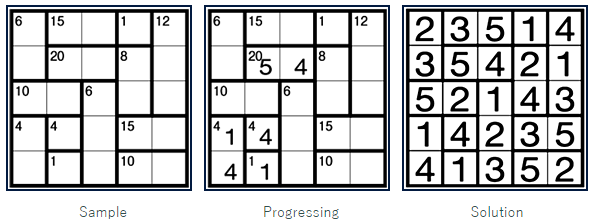
\includegraphics[width=.85\textwidth]{inshi}
\end{figure}

Nous avons choisi deux jeux plutôt différents afin d'augmenter la diversité des structures de données et algorithmes mis en place au sein du projet. Cela nous permet aussi de fournir au client deux exemples de générations et résolutions de problèmes distincts ce qui pourrait être utile pour de prochains projets similaires.\\


\newpage
\section{Description et analyse de l'existant}

\subsection{Analyse du Sudoku fourni}
Nous disposons dans le cadre de ce projet de code source en C similaire à celui qui est attendu de nous pour la résolution et la génération de grilles de Sudoku. Ce code nous a été directement fourni par le client dans le but de nous guider. Il met en place la grande majorité des fonctionnalités que nous devons implémenter mais dans le contexte de la résolution du Sudoku. 

On y observe notamment :
\begin{itemize}
\item L'utilisation de \textit{uint64\_t} pour stocker les valeurs des cellules. Ce type provenant de la bibliothèque standard \textit{stdint.h} permet de définir le nombre de bits qui seront utiliser par une variable. On y retrouvera d'ailleurs \textit{uint\_fast64\_t} qui est un type spécialisé dans la rapidité des opérations.
\item L'implémentation d'une liste chaînée d'une structure conservant chacune la grille d'origine et les modifications qui lui ont été apportées à chaque instant. Cela permet d'effectuer rapidement du backtracking lorsque nécessaire.
\item L'application d'opérations bit à bit au sein d'algorithmes SWAR lors du traitement des données au sein de la grille. Ceci permet d'appliquer une instruction à de multiples données en parallèle afin de réduire le nombre d'opérations nécessaires.\\
\end{itemize}

\subsection{Références relatives à \textit{Hashiwokakero}}
Nous pourrons nous servir d'un court document rédigé par D. Andersson \cite{andersson2009hashiwokakero} qui démontre que le problème \textit{Hashiwokakero} est un problème NP-complet. Nous savons donc qu'il n'existe pas de moyen de trouver une solution à une grille en un temps polynomial. Nous devrons donc tester un ensemble de valeurs sur la grille et effectuer un backtracking lorsque la grille devient impossible à résoudre jusqu'à obtenir une solution, ou alors, jusqu'à que l'on puisse admettre l'absence de solution.\\

\newpage

De même, nous disposons également d'un article de T. Morsink \cite{hashiwokakero2009available} sur le puzzle \textit{Hashiwokakero}. Celui-ci décrit :
\begin{itemize}
\item Les contraintes basiques qui nous permettent de connecter des îles entres elles sans avoir recours au backtracking.
\item Les étapes de résolution effectuées par le solveur réalisé par l'auteur.
\item Les étapes de génération pour implémenter un générateur de nouvelles grilles.
\item Une comparaison des temps pris par le générateur de l'auteur, son solveur et un autre solveur externe pour générer et résoudre des grilles de taille allant de 7x7 à 15x15.\\
\end{itemize}

Afin de représenter les îles et les ponts du jeu \textit{Hashiwokakero}, nous pourrons prendre appui sur une représentation sous forme d'arbre couvrant où chaque noeud représente une île et les ponts sont représentés par des arêtes. Cette implémentation est détaillé au sein de la publication "Rooted Tree and Spanning Tree Constraints" \cite{prosser2006rooted}.

\subsection{Références relatives à \textit{Inshi no heya}}
\textit{Inshi no heya} étant un jeu bénéficiant de moins de popularité que \textit{Hashiwokakero}, il existe peu d'ouvrages concernant les techniques de résolution ou d'autres particularités du puzzle. On peut néanmoins profiter d'un article de J. F. Crook \cite{crook2009pencil} qui décrit en détail l'utilisation d'ensembles préemptifs pour résoudre le Sudoku : des ensembles de valeurs sont attribués à chaque case afin de représenter les valeurs qui peuvent y être assignées. L'application de ceci est utile dans le cas de \textit{Inshi no heya} car, tout comme le Sudoku, on peut déduire les valeurs de certaines cases en se servant des techniques de "naked pairs" et "hidden pairs" qui nous permettent de retrouver le nombre d'une case en fonction des valeurs permises par les autres cases d'une même région (rangée, colonne ou bloc).

\newpage
\section{Description des besoins}

\subsection{Besoins fonctionnels}
\begin{enumerate}
\itemsep1em

\item  \label{besoinF1}Permettre l'affichage d'une grille de jeu :
\begin{enumerate}
\item Concevoir pour chaque puzzle un format d'affichage qui représente tous les éléments qui le compose et qui soit lisible et compréhensible par un utilisateur humain.
\item Implémenter pour chaque programme une fonctionnalité d'affichage permettant d'afficher le puzzle en question sur la sortie standard.
\item \label{besoinF1c}Ces fonctionnalités sont essentielles au bon fonctionnement du programme du fait de leur nécessité pour vérifier l'exécution des autres fonctionnalités. Cela sera assuré par l'utilisation de grilles de test dont les sorties sur console et sur fichier auront été prédéterminées.
\end{enumerate}

\item \label{besoinF2}Permettre la lecture de grilles enregistrées dans des fichiers :
\begin{enumerate}
\item \label{besoinF2a}Définition d'un format de représentation des grilles pour chaque jeu optimisé pour la lecture par ordinateur (figure \ref{fig:inshiTemplate}). Ce format peut donc être différent du format de représentation destiné à l'affichage.
\item \label{besoinF2b}Permettre à chaque programme de lire les fichiers du format qui lui correspond et de convertir les données lues en une structure de données utilisable par le reste du programme via un parseur que nous implémenterons.
\item De part la nature du programme, la lecture des fichiers est un besoin essentiel de ce projet. Le bon fonctionnement de cela sera aussi assuré par la lecture de grilles dont les valeurs qui devront être lues par le programmes seront prédéterminées.
\end{enumerate}

\begin{figure}[H]
\caption{Prototype de format de fichier pour \textit{Inshi no Heya} et sa grille correspondante.}
\label{fig:inshiTemplate}
\centering
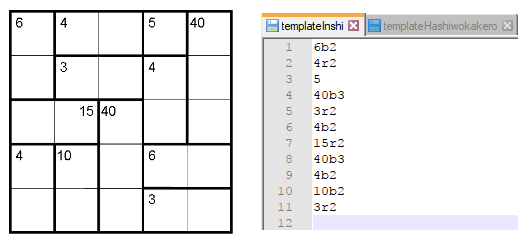
\includegraphics[width=.85\textwidth]{inshiTemp}
\end{figure}

\item \label{besoinF3} Mettre en place, pour chaque jeu, un système de résolution de grilles :
\begin{enumerate}
\item La résolution s'effectuera en étapes dans l'ordre suivant, similaire en exécution à un solveur SAT, afin d'améliorer sa rapidité :
\begin{itemize}
\item Détermination des éléments évidents de la grille de jeu.
\item Construction des variables de la grille dont les valeurs restent à déterminer.
\item Recherche d'une valuation de ces variables qui valide la grille.
\end{itemize}
\item La résolution devra proposer une solution à chaque grille qui lui est fournie, et ce, que la grille admette une unique solution ou plusieurs.
\item La résolution devra se terminer et afficher un message correspondant si la grille fournie n'admet aucune solution.
\item La résolution devra se terminer et afficher un message correspondant si la grille fournie est dans un format incorrect.
\item \label{besoinF3e} Il sera possible d'afficher à chaque étape de la résolution l'état actuel de la grille.
\item La validité de la résolution sera vérifiée à l'aide de grilles de tests dont les résultats auront été prédéterminés.
\item La résolution est un point essentiel du programme. Le suivi des étapes n'est pas nécessaire au bon fonctionnement du programme, il est considéré comme conditionnel.
\end{enumerate}

\item \label {besoinF4} Mettre en place, pour chaque jeu, un système de génération de grilles :
\begin{enumerate}
\item Le programme générera par défaut une grille ayant au moins une solution qu'il affichera à la sortie standard.
\item \label {besoinF4b}L'utilisateur aura la possibilité de décider si la grille générée ne doit admettre qu'une unique solution. 
\item \label {besoinF4c}Permettre la sauvegarde des grilles générées dans des fichiers au même format que celui utilisé pour la lecture de grilles en entrée. 
\item Diverses grilles générées seront résolues à la main afin de vérifier la validité de la génération.
\item La génération des grilles et leur sauvegarde étant réutilisées dans la résolution sont des fonctionnalités essentielles. La génération d'une grille avec une unique solution est une amélioration de la génération, elle est conditionnelle.
\end{enumerate}

\item \label {besoinF5} Mettre en place une taille de grille variable pour chaque jeu :
\begin{enumerate}
\item Définir les dimensions minimums et maximums qui seront supportées par les structures de données utilisées.
\begin{itemize}
\item Pour \textit{Hashiwokakero}, le minimum valide est une grille 3x1 (ou bien 1x3). Le maximum dépendra de notre implémentation mais une taille idéale serait de 64x64.
\item Pour \textit{Inshi no heya}, le minimum valide est une grille 1x1. Le maximum sera fortement limité par les types utilisés au sein de l'implémentation car la valeur attribuée à une salle est, au pire des cas, $N!$ où N est la taille de la grille. On remarquera que un \textit{unsigned long long} peut généralement stocker des valeurs allant jusqu'à $1.84*10^{19}$, ce qui est inférieur à $21!$. On essayera donc à priori de limiter la taille des grilles, ou bien la taille des salles qui les composent, à 20 cases.
\end{itemize}
\item Détecter automatiquement les dimensions des grilles fournies aux programmes.
\item Permettre de choisir les dimensions désirées lors de la génération d'une nouvelle grille.
\item La robustesse du programme doit être assurée : il ne doit pas être possible d'aller aux delà des bornes déterminées pour les dimensions.
\item Pour chacun des programmes, des grilles de test correspondant aux limites des dimensions seront utilisées afin de vérifier la correspondance de la résolution à des résultats préalablement déterminés.
\item Pour chacun des programmes, la validité des grilles générées aux limites des dimensions sera vérifié par la résolution de ces grilles.
\item Ces fonctionnalités de scalabilité sont essentielles.
\end{enumerate}

\end{enumerate}


\subsection{Besoins non fonctionnels}
\begin{enumerate}
\itemsep1em

\item  Un besoin essentiel du projet est que chacun des deux jeux de logique fera l'objet d'un fichier exécutable permettant de réaliser les opérations de résolution et de génération correspondant à son jeu.

\item \label {besoinNF2} Les grilles de jeu pouvant être de grande taille (3.1.\ref{besoinF5}), la résolution (3.1.\ref{besoinF3}) et la génération (3.1.\ref{besoinF4}) doivent être optimisées : 
\begin{enumerate}
\item Utiliser un langage de programmation faible en consommation de mémoire et efficace en temps de calcul. Il a donc été convenu avec le client lors du premier entretien que les programmes seraient implémentés en C dans la mesure du possible.
\item Mettre en place des algorithmes de résolution optimaux afin de déterminer tous les éléments certains d'une grille en moins d'une seconde.
\item \label {besoinNF2c}Utiliser de manière intensive des algorithmes SWAR. Cela désigne le fait d'appliquer une seule instruction sur de multiples données contenu dans un registre. Dans notre cas, on utilisera ces algorithmes pour réduire le temps de calcul en regroupant des données et en utilisant une seule instruction sur celles-ci ce qui est plus rapide que de réitérer la même instruction au sein d'une boucle.
\item Il faut se servir de structures de données concises utilisant des types optimisés pour du traitement bit à bit tels que \textit{uint64\_t} et \textit{uint\_fast32\_t}. 
\item \label {besoinNF2e}Exécuter plusieurs threads afin de répartir les tâches effectuées lors de la résolution et la génération de grilles. Ceci a été vu comme une fonctionnalité supplémentaire pouvant être ajoutée au projet afin de l'améliorer au delà de ce qui est attendu.
\item On doit nécessairement utiliser un langage de programmation efficace. Des comparaisons seront établies entre les différents algorithmes implémentés afin de déterminer leur efficacité. 
\item Il est essentiel d'utiliser des algorithmes de résolution optimaux et des algorithmes SWAR ainsi qu'utiliser des structures de données concises. L'utilisation de plusieurs threads est optionnelle.
\end{enumerate}

\item S'assurer de la robustesse de la lecture des fichiers d'entrée (3.1.\ref{besoinF2}):
\begin{enumerate}
\item En cas d'erreur mineure dans le fichier qui n'empêche pas sa compréhension, permettre de continuer la lecture en corrigeant le défaut.
\item En cas d'erreur majeure dans le fichier qui rend la grille invalide, afficher un message d'erreur avant de mettre fin au programme.
\item Ce besoin n'étant pas nécessaire à l'exécution du programme, il est conditionnel au projet.
\end{enumerate}

\item Implémenter pour chaque programme la possibilité d'enregistrer la représentation de la grille dans un fichier, particulièrement pour les cas où la grille aurait des dimensions excessives pour s'afficher correctement en console. Ce besoin est conditionnel.
\item  Chaque programme devra disposer de plusieurs options d'exécution :
\begin{enumerate}

\item Comportement par défaut (3.1.\ref{besoinF3}):
\begin{itemize}
\item Prend un paramètre : le nom du fichier contenant la grille à résoudre.
\item Lance la résolution d'une grille contenue dans un fichier et affiche en sortie standard la grille initiale puis la grille résolue.
\item Ceci est, bien évidemment, essentiel au projet.\\
\end{itemize}

\item \textit{-generate} (3.1.\ref{besoinF4}):
\begin{itemize}
\item Prend un paramètre : la taille de la grille à générer.
\item Permet de générer une nouvelle grille avec au moins une solution dont la taille est déterminée par l'utilisateur.
\item Est compatible avec toutes les autres options d'exécution.
\item Cette fonctionnalité est un des points clés du programme et est donc essentielle.\\
\end{itemize}

\item \textit{-strict} (3.1.\ref{besoinF4b}):
\begin{itemize}
\item Force la grille générée à n'avoir qu'une unique solution.
\item Cette option doit être utilisée avec l'option de génération et est compatible avec toutes les autres options d'exécution.
\item Tel que vu précédemment, cette fonctionnalité est conditionnelle.\\
\end{itemize}

\item \textit{-save}(3.1.\ref{besoinF4c}) :
\begin{itemize}
\item Prend un paramètre : le nom du fichier de sortie.
\item Si le format de fichier d'entrée et différent de celui utilisé pour l'affichage de grilles, cette option permet d'enregistrer une grille générée au format d'entrée.
\item Cette option doit être utilisée avec l'option de génération et est compatible avec toutes les autres options d'exécution.
\item Cette fonctionnalité est essentielle à implémenter pour les tests de génération.\\
\end{itemize}

\item \textit{-output} (3.1.\ref{besoinF1c}):
\begin{itemize}
\item Prend un paramètre : le nom du fichier de sortie.
\item Permet d'enregistrer un affichage compréhensible de la grille résolue ou générée dans un fichier sans l'afficher au préalable en sortie standard.
\item Est compatible avec toutes les autres options d'exécution.
\item Cette fonctionnalité est essentielle.\\
\end{itemize}

\item \label {besoinNF5f}\textit{-verbose} (3.1.\ref{besoinF3e}):
\begin{itemize}
\item Permet d'afficher chaque étape de la résolution ou de la génération de la grille.
\item Est compatible avec toutes les autres options d'exécution.
\item Tel que vu précédemment, cette fonctionnalité est conditionnelle.\\
\end{itemize}

\item \textit{-help} :
\begin{itemize}
\item Permet d'afficher des informations sur le programme et ses options d'exécution. 
\item Cette option peut être utilisée avec toute autre option. 
\item Ceci apporte des informations supplémentaires non requis pour l'utilisation du programme, son implémentation est donc conditionnelle.\\
\end{itemize}

\item \textit{-version} :
\begin{itemize}
\item Permet d'afficher la version courante du programme.
\item Cette option peut être utilisée avec toute autre option. 
\item Ceci apporte des information supplémentaires non nécessaires à l'utilisation du programme, son implémentation est donc conditionnel.\\
\end{itemize}

\end{enumerate}


\item La réalisation du projet devra respecter le calendrier prévisionnel de l'UE Projet de Programmation :
\begin{enumerate}
\item \label {besoinNF6a}Une première version du livrable devra être fournie pour le 16 février.
\item Un audit lors du 28 février.
\item \label {besoinNF6c}Une version final du livrable ainsi qu'un mémoire devra être fournie pour le 5 avril.
\item Une soutenance aura lieu le 11 avril.
\end{enumerate}

\end{enumerate}

\newpage
\section{Diagrammes de Gantt}

\subsection{Documentation auxiliaire}
\vspace{6em}

\begin{figure}[H]

\begin{ganttchart}[hgrid=dotted, vgrid={*2{draw=none}, dotted}]{1}{15}
\gantttitle{Semaine}{15} \\
\gantttitlelist{1,...,15}{1} \\

\ganttbar[name=d1]{Rencontre initiale avec le client}{2}{2} \\
\ganttlinkedbar[name=d2]{Analyse des besoins}{2}{4} \\
\ganttlinkedmilestone[name=d3]{Remise de l'analyse des besoins}{4} \\

\ganttmilestone[name=d4]{Audit}{8} \\
\ganttlinkedbar[name=d5]{Remaniement de l'analyse des besoins}{9}{9} \\

\ganttbar[name=d6]{Rédaction du mémoire}{9}{13} \\
\ganttlinkedmilestone[name=d7]{Remise du mémoire}{14} \\
\ganttlinkedmilestone[name=d8]{Soutenance}{15}


\end{ganttchart}

\caption{Planning de la rédaction des documents propres au projet.}
\label{fig:ganttDocs}
\centering

\end{figure}

\newpage
\subsection{Réalisation de l'implémentation}

La répartition des tâches suivante s'applique à chacun des deux puzzles de manière identique. Les deux programmes seront développés en parallèle. \newline

\begin{figure}[H]

\begin{ganttchart}[hgrid=dotted, vgrid={*2{draw=none}, dotted}]{1}{15}
\gantttitle{Semaine}{15} \\
\gantttitlelist{1,...,15}{1} \\

\ganttbar[name=p1]{Conception des formats de fichiers (3.1.\ref{besoinF2a})}{3}{3} \\
\ganttlinkedbar[name=p2]{Lecture de fichiers d'entrée avec robustesse (3.1.\ref{besoinF2b})}{4}{4} \\
\ganttbar[name=p3]{Affichage et sortie sur fichier(3.1.\ref{besoinF1})}{4}{4} \\
\ganttlinkedbar[name=p4]{Mise en place d'algorithmes de résolution(3.1.\ref{besoinF3})}{5}{5} \\
\ganttlinkedbar[name=p5]{Optimisation via algorithmes SWAR(3.2.\ref{besoinNF2c})}{5}{6} \\
\ganttlinkedmilestone[name=p6]{Première release(3.2.\ref{besoinNF6a})}{6} \\
\ganttlinkedbar[name=p7]{Finalisation de l'optimisation de la résolution(3.2.\ref{besoinNF2})}{7}{8} \\

\ganttbar[name=p8]{Génération de grilles(3.1.\ref{besoinF4})}{6}{9} \\
\ganttlinkedbar[name=p9]{Optimisation dé génération(3.2.\ref{besoinNF2}}{10}{11} \\
\ganttlinkedbar[name=p10]{Génération de grilles à solution unique(3.1.\ref{besoinF4b}}{12}{13} \\

\ganttbar[name=p11]{Implémentation de la verbosité(3.2.{\ref{besoinNF5f}})}{11}{12} \\
\ganttlinkedbar[name=p12]{Implémentation du multithreading(3.2.\ref{besoinNF2e})}{13}{14} \\
\ganttlinkedmilestone[name=p13]{Release finale(3.2.\ref{besoinNF6c})}{14}

\ganttlink[link mid=.25]{p1}{p3}
\ganttlink[link mid=.75]{p2}{p4}

\end{ganttchart}

\caption{Distribution de la charge de travail au cours du semestre.}
\label{fig:ganttProjet}
\centering

\end{figure}


\newpage
\bibliography{biblio}


\end{document}